\chapter{Functional Methods in Quantum Field Theory}\label{chap:QFT}
This chapter introduces a treatment of quantum field theory using functional methods. The main goal is to become familiar with the physical concepts and the notation used throughout this work and to derive the flow equation for the average effective action, introduced by Christof Wetterich in 1993 \cite{Wetterich1992}. 
For the derivation of the flow equation we are following \cite{Gies2006, PawlowskiNPgaugeLecture}.

\section{Generating Functionals and Correlation Functions}
Consider a theory setting of $N$ real scalar fields $\varphi_a(x), a \in \{1,\dots,N\}$ in $d$-dimensional Euclidean space. The corresponding partition sum in presence of sources $J_a(x)$ reads
\begin{align}
	Z[J] = \frac{1}{\mathcal{N}} \int \D\varphi \operatorname{e}^{-\S + J\cdot\varphi}.
	\label{eqn:partition}
\end{align}
The action $\mathcal{S}$ is specified together with an ultraviolet cutoff scale $\Lambda$, later being the momentum scale where we initialize the flow equations and some normalization factor $\mathcal{N}$.\\
In this notation, the scalar product sums over field components and integrates over all space,
\begin{align}
	J\cdot\varphi = \int_x J_a(x) \ \varphi_a(x) = \int_p \tilde{J}_a(p) \ \tilde{\varphi}_a(p),
\end{align}
with
\begin{align}
\int_x = \int_{\mathbb{R}^d} \dd^d x \qquad \text{and} \qquad \int_p = \int_{\mathbb{R}^d} \frac{\dd^d p}{(2\pi)^d}.	
\end{align}

The partition sum $Z[J]$ is called a \textit{generating functional}. It directly allows us to compute field expectation values
\begin{align}
	\phi := \cf{\varphi} = \eval{\frac{1}{Z}\frac{\delta Z}{\delta J}}_{J=0} = \int \D\varphi \ \varphi \ \operatorname{e}^{-\S + J\cdot\varphi}
\end{align}
and higher order correlation functions
\begin{align}
\cf{\varphi(x_1) \cdots \varphi(x_n)} := \cf{\varphi^n} = \frac{1}{Z}\eval{\frac{\delta^n Z}{\delta^n J}}_{J=0} = \int \D\varphi \ \overbrace{\varphi_1 \cdots \varphi_n}^{:= \ \varphi^n} \ \operatorname{e}^{-\S + J\cdot\varphi}
\end{align}
via functional differentiation. This means, we are basically able to compute all contributing Feynman diagrams for our theory setting, if we have knowledge of its corresponding (grand) canonical partition sum. \\
 For a more efficient description of the theory in terms of only the \textit{connected} correlation functions, we define the \textit{Schwinger functional} $W[J]$ as the logarithm of $Z[J]$,  
\begin{align}
W[J] = \ln Z[J].
\label{eqn:Schwinger}
\end{align}
It is the generating functional for the connected correlation functions. The normalization factor $\mathcal{N}$, introduced in (\ref{eqn:partition}) enters here as an additive constant, which drops out for all higher order correlation functions, except for the zero-point function. This term is connected to the thermodynamic quantities of the system and becomes important, when external parameters such as temperature, volume or the chemical potential are varied. For the case of quantum gravity, it is linked to the cosmological constant $\Lambda$. Nevertheless, in general we are only interested in correlation functions with $n\geq 1$ and therefore we drop this term.\\
Consider for example the connected two-point function $G_{ab}(x,y) = G_{\alpha\beta}$\footnote{To save on notation, we introduce collective indices $\alpha = (x,a)$ or $(q,a)$ in momentum space.}, known as the propagator, correlating the field $\varphi_a$ at spacetime point $x$ with the field $\varphi_b$ at $y$,
\begin{equation}
\begin{aligned}
	G_{\alpha\beta} &= \frac{\delta^2W[J]}{\delta J_{\alpha}\delta J_{\beta}} = \frac{\delta}{\delta J_{\alpha}}\left(\frac{1}{Z}\frac{\delta Z}{\delta J_{\beta}}\right)  \\[10pt]
				&= \frac{1}{Z}\left(\frac{\delta^2Z}{\delta J_{\alpha}\delta J_{\beta}}\right) - \frac{1}{Z^2}\left(\frac{\delta Z}{\delta J_{\alpha}}\right)\left(\frac{\delta Z}{\delta J_{\beta}}\right)\\[10pt]
				&= \cf{\varphi_{\alpha}\varphi_{\beta}} - \phi_{\alpha}\phi_{\beta} = \cf{\varphi_{\alpha}\varphi_{\beta}}_{\text{c}}. 
\end{aligned}
\label{eqn:G_connected}						
\end{equation}
The propagator is the key object in functional approaches to quantum field theory. It depends on the chosen background via $J$. \\
It is still possible to make our computations even more efficient, because $W[J]$ still contains some redundant information. Connected correlation functions can be separated into so-called one-particle irreducible (1PI) and one-particle reducible ones. The 1PI correlation functions are those, whose corresponding Feynman diagrams can \textit{not} be separated into two disconnected ones by cutting a single internal line. As an example, contributing 1PI and reducible diagrams to the connected four-point function for Yukawa theory are depicted in figure (\ref{fig:1PI_Yukawa}). \\
\begin{figure}[t]
\centering
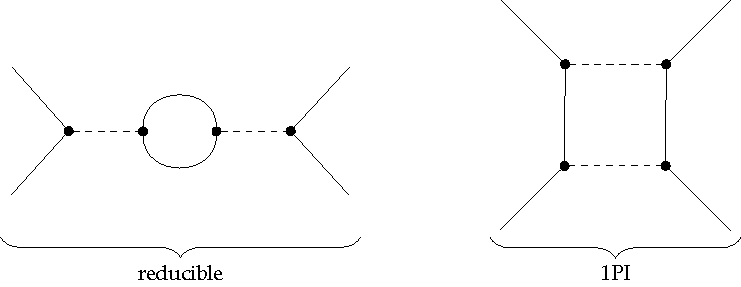
\includegraphics[width=0.8\textwidth]{figs/TikZ/1PI_Yukawa}
\caption[Contributing one-particle reducible and 1PI diagrams to the four-point-function in Yukawa theory]{Contributing one-particle reducible and 1PI diagrams to the four-point-function in Yukawa theory, inspired by \cite{FloerchingerWetterichQFT}.}	
\label{fig:1PI_Yukawa}
\hrulefill
\end{figure}
The generating functional for the  1PI correlation functions, the \textit{effective action} $\Gamma$, is obtained from the Schwinger functional via a Legendre transformation, 
\begin{equation}
	\Gamma[\phi]=\sup _{J}\left\{\int_{x} J(x) \phi(x)-W[J]\right\}=\int_{x} J_{\mathrm{sup}}(x) \phi(x)-W\left[J_{\mathrm{sup}}\right],
\label{eqn:Def_Gamma}
\end{equation}
where $J_{\mathrm{sup}}$ has to be understood as a field-dependent current $J_{\mathrm{sup}}[\phi]$. In the following, we will drop the subscript, its meaning is implicitly understood. 
The quantum equation of motion derived from $\Gamma$ reads
\begin{align}
	J(x) = \frac{\delta\Gamma[\phi]}{\delta\phi(x)}.
	\label{eqn:quantum_eom}
\end{align}
It allows us to understand the dynamics of field expectation values, taking the effects of all quantum fluctuations into account.
From a physical point of view, the effective action $\Gamma$ is the quantum analogue of the classical action $\mathcal{S}$. The performed Legendre transformation leads us to a mean field description of our theory with $\phi = \cf{\varphi}$ on a given background, as introduced before. The symmetries of the classical action are in general still present in the effective action.\\
In terms of the effective action, higher order correlation functions are again obtained by performing functional derivatives, but now w.\,r.\,t. the mean field $\phi$,
\begin{align}
	\Gamma^{(n)}\left(x_{1}, \ldots, x_{n}\right)=\frac{\delta^{n} \Gamma}{\delta \phi\left(x_{1}\right) \cdots \delta \phi\left(x_{n}\right)}.
\end{align}
With the definition of the effective action (\ref{eqn:Def_Gamma}), we find
\begin{equation}
	\operatorname{e}^{-\Gamma[\phi]}=\int_{\Lambda} \mathcal{D} \varphi \exp \left(-\mathcal{S}[\phi+\varphi]+\int_x \frac{\delta \Gamma[\phi]}{\delta \phi(x)} \varphi(x)\right).
\end{equation}  
The solution of such functional integro-differential equations is highly non-trivial. To solve this problem, we want to make use of the Functional Renormalization Group. The general idea of this approach is to introduce a scale-dependent action $\Gamma_k$, interpolating between the bare, microscopic action $\mathcal{S}$ and the full quantum effective action $\Gamma$. A more formal motivation and a derivation of the equation governing this interpolation process is presented in the next section.   
 \section{Functional Renormalization Group}
The Functional Renormalization Group (FRG) is a mathematical tool, allowing us to investigate the dynamics of physical systems on different energy (momentum) scales. This idea is based on a continuous version of Leo P. Kadanoff's block spin model on the lattice \cite{Kadanoff1966} and was developed by Kenneth G. Wilson in 1971 \cite{Wilson1971}. It aims at solving the theory by integrating successively momentum shell by momentum shell, being the reason why the path integral approach to quantum field theory provides a suitable framework. The main advantage of the FRG approach is, that no regularization or renormalization procedure has to be applied. The latter one is already implemented systematically, which secures the self-consistency of the approach. As this section is only supposed to introduce the basics of the FRG, we refer the interested reader to more complete reviews, e.\,g. \cite{Pawlowski2005, Gies2006}, particularly for applications in different areas of physics.

As a first step towards a FRG equation we need to introduce an infrared cutoff scale $k$ in our theory, below which the modes are not integrated out. A common way to introduce such a scale is by  adding a scale-dependent cutoff term $\Delta\mathcal{S}_k$ in the definition of the partition sum (\ref{eqn:partition}) and therefore automatically also in the definition of the Schwinger functional (\ref{eqn:Schwinger}):
\begin{align}
W_{k}[J]=\ln Z_{k}[J]=\ln \int \mathcal{D} \varphi  \operatorname{e}^{-\mathcal{S}[\varphi]+J \cdot \varphi-\Delta \mathcal{S}_{k}[\varphi]}.
\label{eqn:Wk}
\end{align}
The physical scale $k$ we introduced here is known as \textit{renormalization scale} and has units of inverse length, meaning large $k$ correspond to small distances and vice versa. The cutoff term $\Delta\mathcal{S}_k$ is a quadratic functional depending on the field $\varphi$:
\begin{align}
	\Delta \mathcal{S}_{k}[\varphi]=\frac{1}{2} \varphi \cdot R_{k} \cdot \varphi=\frac{1}{2} \int_{x, y} \varphi_{\alpha} \ R_{k, \alpha\beta} \ \varphi_{\beta}.
\end{align}
The function $R_k$ is called \textit{regulator}. It plays an important role for this formulation of quantum field theory. The regulator is chosen such that only the propagation for momentum modes with $p^2 \lesssim k^2$ is suppressed. The most important physical limits are summarized in the following:
\begin{align}
	R_{k}(p^2) \rightarrow\left\{\begin{array}{ll}{k^{2}} & {\text { for } p \rightarrow 0} \\ {0} & {\text { for } p \rightarrow \infty} \\ {0} & {\text { for } k \rightarrow 0} \\ {\infty} & {\text { for } k \rightarrow \Lambda}\end{array}\right.
\label{eqn:regulator_limits}
\end{align}
A convenient choice of the regulator is given by
\begin{align}
	R_k(p^2) = p^2 \cdot r_k(y),
\end{align}
with $ y := \frac{p^2}{k^2}$, and a dimensionless regulator shape function $r_k$, only depending on the dimensionless momentum ratio $y$. There is a plethora of different types of shape functions, but for the computations performed in this work we restrict ourselves to a class of rather simple, so-called Litim-type regulators with shape functions
\begin{align}
r_k(y) = \left(\frac{1}{y} - 1\right)\theta(1-y),
\label{eqn:Litim}	
\end{align}
where $\theta$ is the Heaviside step function. This class of \textit{sharp} regulators is a good choice for finding analytic FRG equations in simple approximations. For numerical approaches, exponential regulators such as depicted in figure (\ref{fig:exp_regulator}) are well suited.\\
\begin{figure}[t]
\centering
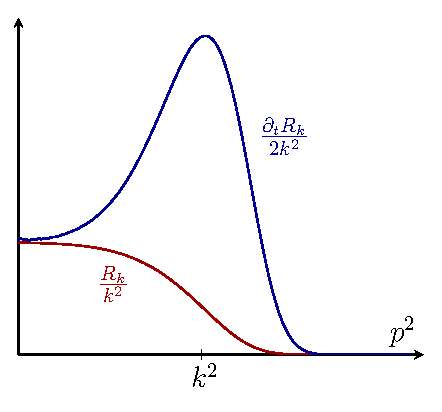
\includegraphics[width=0.4\textwidth]{figs/Plots/regulator_plot}
\caption[Shape of a typical exponential regulator function $R(p^2)$ and its derivative w.\,r.\,t. the RG time $t$.]{Shape of a typical exponential regulator function $R(p^2)$ and its derivative w.\,r.\,t. the RG time $t$. The regulator has a finite value for momenta smaller than $k^2$ and therefore acts as a suppressing mass term. The peak of $\partial_tR_k$ around $k^2=p^2$ clearly shows the implementation of Wilsons idea of shell-wise momentum integration.}	
\label{fig:exp_regulator}
\hrulefill
\end{figure}
At this point it is quite convenient to introduce the \textit{RG time} $t$ as
\begin{align}
	t = \ln\left(\frac{k}{\Lambda}\right) \qquad \longrightarrow\qquad \partial_t = \frac{\partial}{\partial\ln(k/\Lambda)} = \frac{k}{\Lambda}\frac{\partial}{\partial(k/\Lambda)} = k \partial_k,
\end{align}
where $\Lambda$ is a fixed reference scale. Usually one chooses the ultraviolet cutoff scale, where the flow is initialized.\\
In this setting, (\ref{eqn:Wk}) provides a good starting point for solving the theory by successively lowering the cutoff scale $k$ infinitesimally and integrating out all momentum modes $\varphi_{p\approx k}$. This procedure can be formalized by taking a scale derivative of our scale-dependent functional (\ref{eqn:Wk}):
\begin{equation}
\begin{aligned} \partial_{t} W_{k}[J] &=-\frac{1}{2} \int \mathcal{D} \varphi \ \varphi(-p) \partial_{t} R_{k}(p) \varphi(p) \operatorname{e}^{-\mathcal{S}[\varphi]+ J \cdot\varphi - \Delta \mathcal{S}_{k}[\varphi]} \\ &=-\frac{1}{2} \int_p \partial_{t} R_{k}(p) G_{k}(p)+\partial_{t} \Delta S_{k}[\phi], 
\label{eqn:dtW}
\end{aligned}
\end{equation}
where we used the definition of the connected propagator:
\begin{equation}
G_k = \frac{\delta^2 W_k[\phi]}{\delta\phi(x)\delta\phi(y)}.
\label{eqn:Gk}
\end{equation}
The \textit{flowing} or \textit{effective average action} $\Gamma_k$ is then again defined via a modified Legendre transformation, including the insertion of $\Delta S_k$:
\begin{equation}
	\Gamma_{k}[\phi]=\sup _{J}\left(\int_x J(x) \phi(x)-W_{k}[J]\right)-\Delta S_{k}[\phi].
\end{equation}
This yields the modified, scale-dependent quantum equation of motion:
\begin{align}
	J(x) = \frac{\delta\Gamma_k[\phi]}{\delta\phi(x)} + \left(R_k\phi\right)(x).
\end{align}
Compared to the scale-independent version (\ref{eqn:quantum_eom}), we find an additional, regulator dependent term, but with the properties of the regulator presented in (\ref{eqn:regulator_limits}) in mind, we see that in the limit $k\rightarrow 0 $ the initial equation of motion is restored.
We find
\begin{equation}
	\frac{\delta J(x)}{\delta \phi(y)}=\frac{\delta^{2} \Gamma_{k}[\phi]}{\delta \phi(x) \delta \phi(y)}+R_{k}(x, y).\label{eqn:dJdphi}
\end{equation}
With the help of these relations we are able to show that 
\begin{equation}
\begin{aligned} \delta\left(x-x^{\prime}\right) =\frac{\delta J(x)}{\delta J\left(x^{\prime}\right)}&=\int_y \frac{\delta J(x)}{\delta \phi(y)} \frac{\delta \phi(y)}{\delta J\left(x^{\prime}\right)} \\[10pt] &=\int_y\left(\Gamma_{k}^{(2)}[\phi]+R_{k}\right)(x, y) \ G_{k}\left(y-x^{\prime}\right).
\end{aligned}
\end{equation}
Here, we used (\ref{eqn:dJdphi}) and the definition of $G_k$ (\ref{eqn:Gk}). 
This yields the following important identity:
\begin{equation}
	G_k = \left(\Gamma_k^{(2)} + R_k\right)^{-1}.
	\label{eqn:inverse_prop_identity}
\end{equation}
Altogether, we arrive at the \textit{flow equation}, a.\,k.\,a. the \textit{Wetterich equation} for the average effective action:
\begin{equation}
\begin{aligned}
\partial_t \Gamma_k[\phi] &\overset{\phantom{(\ref{eqn:dtW})}}{=} -\partial_t W_k +\int\left(\partial_t J\right) \phi - \partial_t \Delta S_k[\phi] = - \partial_t W_k[J] - \partial_t \Delta S_k[\phi] \\[5pt] 
&\overset{(\ref{eqn:dtW})}{=} \frac{1}{2} \int_p G_{k}(p) \ \partial_{t} R_{k}(p)\\[5pt]
&\overset{(\ref{eqn:inverse_prop_identity})}{=}\frac{1}{2} \operatorname{STr}\left[\left(\Gamma_{k}^{(2)}[\phi]+R_{k}\right)^{-1}\partial_{t} R_{k}\right].
\end{aligned}
\label{eqn:Wetterich}
\end{equation}
The supertrace $\operatorname{STr}$ sums over all internal indices and integrates over momentum space. For Grassmann fields, it also involves the inclusion of a minus sign. We will drop the $\operatorname{S}$ for the rest of this work, its meaning should be understood implicitly.
The flow equation can be represented diagrammatically as a $1$-loop equation:
\begin{figure}[H]
\centering
\begin{gather}
\begin{aligned}
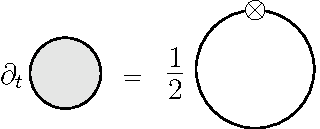
\includegraphics[scale=1.1]{figs/TikZ/wetterich_equation}
\end{aligned}
\end{gather}
\end{figure}
\vspace{-0.7cm}
The full propagator $\left[\Gamma_k^{(2)} + R_k\right]^{-1}$ is represented as usual as a single, double, dashed etc. line, dependent on the field content.
The crossed circle $\otimes$ denotes the insertion of the respective regulator or more precisely its derivative w.\,r.\,t. the RG time $t$. Here $\partial_{t} R_{k, ij}(p, q)=\partial_{t} R_{k}(p^2)(2 \pi)^{d} \  \delta_{i j} \ \delta(p-q)$ and therefore the trace on the r.\,h.\,s. effectively sums over just one index $i$ and integrates over one loop momentum $p$. \\
\begin{figure}[t]
\centering
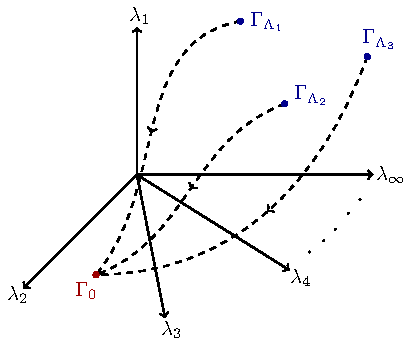
\includegraphics{figs/TikZ/regulator_dependence}
\caption[Flow of $\Gamma_k$ through infinite-dimensional theory space for different regulators.]{Flow of $\Gamma_k$ through infinite-dimensional theory space for different regulators, inspired by \cite{Gies2006}. Although the trajectories in theory space, governed by the flow equation (\ref{eqn:Wetterich}) may be different, they flow towards the same quantum effective action $\Gamma_{k\rightarrow 0} \equiv \Gamma$.}	
\label{fig:theory_space}
\hrulefill
\end{figure}
It is important to mention, that the Wetterich equation is an \textit{exact} equation, no approximations have been made. The only modification, the implementation of $\Delta S_k$ vanishes in the limit $k\rightarrow 0$. Solutions of the flow equation correspond to trajectories in \textit{theory space}, the space spanned by all (= infinitely many) dimensionless couplings $g_{\alpha}$. The choice of the regulator has direct impact on the exact form of the trajectory. This is often referred to as \textit{scheme dependence}. Nevertheless, for all regulators satisfying the properties (\ref{eqn:regulator_limits}) it is guaranteed, that the flow will lead to the same quantum effective action $\Gamma$. For a visualization of this idea, have a look at figure (\ref{fig:theory_space}).  In principle this means, that $\lim_{k\rightarrow 0}\Gamma_k\equiv\Gamma$, but in most practical cases it is unavoidable to employ truncation schemes to be able to solve the flow equation. A plethora of different truncation schemes has been developed recently, details concerning the most important schemes can be found e.\,g. in the reviews about the FRG we referred to at the beginning of this section. We want to conclude this chapter with a more formal discussion of the concept of theory space, before proceeding to an introduction of the basic concepts of (classical) gravity.
\section{Renormalization Group Flow and Theory Space}
We want to use this section to formalize the concept of theory space we introduced in the last section and to discuss important characteristics of the renormalization group flow such as the beta functions and their zeros, the fixed points of the flow. For this part, we mainly follow \cite{ReuterSaueressig2012}. \\
The theory space is defined as the space spanned by all dimensionless couplings of the theory. To be more precise, it consists of all (action) functionals $A:\Phi \mapsto A[\Phi]$, that are compatible with the imposed symmetries of the theory such as e.\,g. diffeomorphism invariance in the case of (quantum) gravity. \\
The flow equation (\ref{eqn:Wetterich}) defines a vector field $\vec{\beta}$ in theory space whose integral curves are the trajectories $\Gammak$ parametrized by the scale $k$. Assuming the existence of a complete set of basis functionals $\left\{P_{\alpha}[\ \cdot \ ]\right\}$, we can expand $\Gamma_k$ as follows:
\begin{equation}
	\Gamma_{k}[\Phi, \bar{\Phi}]=\sum_{\alpha=1}^{\infty} \bar{g}_{\alpha}(k) P_{\alpha}[\Phi, \bar{\Phi}].
\end{equation}
Here, the expansion coefficients $ \bar{g}_{\alpha}(k)$ are given by the generalized couplings. Inserting this ansatz into the flow equation (\ref{eqn:Wetterich}), yields a set of infinitely many coupled differential equations for the couplings:
\begin{equation}
	k \partial_{k} \bar{g}_{\alpha}(k)=\bar{\beta}_{\alpha}\left(\bar{g}_{1}, \bar{g}_{2}, \cdots ; k\right), \qquad \alpha=1,2, \cdots
\end{equation}
The \textit{beta functions} $\bar{\beta}_{\alpha}\left(\bar{g}_{1}, \bar{g}_{2}, \cdots ; k\right)$  are the components of the vector field $\vec{\beta}$ and arise from an expansion of the trace on the r.\,h.\,s. of the flow equation in terms of the functional basis\footnote{The expansion reads: $\frac{1}{2}\tr{\cdots} = \sum_{\alpha=1}^{\infty} \bar{\beta}_{\alpha}\left(\bar{g}_{1}, \bar{g}_{2}, \cdots ; k\right) P_{\alpha}[\Phi, \bar{\Phi}]$.}. Up to this point, we are still dealing with dimensionful couplings $\bar{g}$, but as mentioned earlier usually the flow equation is expressed in terms of \textit{dimensionless couplings}
\begin{equation}
	g_{\alpha} \equiv k^{-d_{\alpha}} \bar{g}_{\alpha},
\end{equation}
where $d_{\alpha}$ is the canonical mass dimension of the respective coupling. The \textit{essential} couplings\footnote{Essential in this sense means, that they can not be absorbed into the fields via a rescaling.} provide a set of coordinates for the theory space. This allows us to interpret the idea of renormalization theory in a new, geometrical way: We need to construct \enquote{infinitely long} trajectories $\Gammak$, that lie \textit{entirely} in theory space. In this case, the couplings are prevented from diverging and we are able to define a consistent quantum field theory. \newpage
A \textit{fixed point} $g^{*}$ of the flow is a zero point of the vector field $\vec{\beta}$, i.\,e.  $\beta_{\alpha}(g^{*})\equiv 0 \ \forall \alpha$. The existence of such fixed points is crucial for our discussion of Asymptotic Safety as an approach to quantum gravity, based on the concepts we introduced here. \\
\begin{figure}[t]
	\centering
	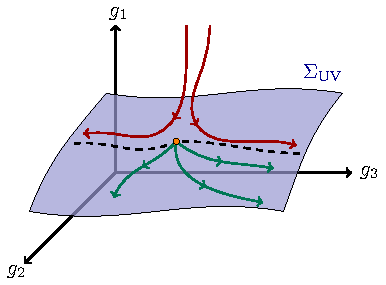
\includegraphics[width=0.5\textwidth]{figs/TikZ/hypersurface}
	\caption[Visualization of a fixed point with its corresponding UV hypersurface $\Sigma_{\mathrm{UV}}$ in theory space.]{Visualization of a fixed point $g^{*}$ (orange dot) with its corresponding UV hypersurface $\Sigma_{\mathrm{UV}}$ and trajectories starting at $g^{*}$ (green) in theory space. The flow points towards the IR. Trajectories starting off the surface (red) are pulled towards the FP along the irrelevant direction (here: $g_1$) until  the IR repulsive directions $g_2$ and $g_3$ dominate and drive the flow away from $g^{*}$. This figure is inspired by \cite{Eichhorn2018}.}\label{fig:hypersurface}
	\hrulefill
\end{figure}
In general, one distinguishes different classes of fixed points. The \textit{Gaussian} or \textit{non-inter-acting} fixed points  (GFP) are classified by $g^{*}_{\alpha}=0 \ \forall\alpha$. This class of fixed points is relevant for perturbation theory, where the limit $k\rightarrow\infty$ is taken at such a GFP\footnote{E.\,g. in Yang-Mills theory, the concept of \textit{Asymptotic freedom}, where the couplings tend to zero in the limit $k\rightarrow\infty$, is based on the existence of an UV attractive Gaussian fixed point, rendering the theory perturbatively renormalizable \cite{GrossWilczek1973}.}. If at least one of the couplings $g^{*}_{\alpha}\neq 0$, the fixed point is classified as \textit{Non-Gaussian} or \textit{interacting} (NGFP). The idea of Asymptotic Safety relies on the existence of such a NGFP, rendering the theory \enquote{safe} from divergences in the ultraviolet (UV) regime. An important characteristic of a fixed point is its stability or more precisely if it is \textit{attractive} or \textit{repulsive} for near RG trajectories. Additionally one distinguishes between infrared ($k\rightarrow0$) and ultraviolet ($k\rightarrow\infty$) attractive (repulsive) fixed points. To analyze this behavior, the flow near a fixed point is linearized, i.\,e.
\begin{equation}
	\partial_{t} g_{\alpha}(k)=\sum_{j=1}^{\infty} B_{\alpha j}\left(g_{j}-g_{j}^{*}\right),
	\label{eqn:linearized_flow}
\end{equation}
where we defined the \textit{stability matrix} \ $\mathbf{B} = B_{\alpha j} = \partial_j\beta_{\alpha}(g^{*}_{\alpha}) $. The solution of the differential equation (\ref{eqn:linearized_flow}) reads:
\begin{equation}
	g_{\alpha}(k)=g_{\alpha}^{*}+\sum_{j=1}^{\infty} C_{j} V_{\alpha}^{j}\left(\frac{k}{k_{0}}\right)^{\theta_{j}}.
\end{equation}
Here, the $V^{j}$ are the eigenvectors of the stability matrix with eigenvalues $\theta_j$ a.\,k.\,a. \textit{critical exponents}. In general, the $\theta_{j}$, are complex numbers. We use the real part of the critical exponents to classify the coupling as \textit{relevant} (= attractive) or \textit{irrelevant} (= repulsive):
\begin{align}
	g^{*}_{\alpha} \ \text{ is } \left\{\begin{array}{ll}{\text{relevant }} & {\text { for } \ \mathfrak{Re}\left(\theta_j\right) > 0} \\[10pt] {\text{irrelevant }} & {\text { for } \  \mathfrak{Re}\left(\theta_j\right) < 0} \\ \end{array}\right..
\end{align}
Fixed points with critical exponents $\theta_{j}=0$ are called \textit{marginal}. Based on this classification, it follows quite naturally to define an UV (or IR)  \textit{critical hypersurface} $\Sigma_{\mathrm{UV}}$ in theory space for a NGFP, consisting of all points that are pulled into the NGFP for increasing $k$. The dimension of $\Sigma_{\mathrm{UV}}$ is equal to the number of UV relevant couplings. This means, that trajectories lying on such a hypersurface tend to flow towards the fixed point in the UV limit. To visualize this idea, a schematic sketch of such a hypersurface in a $3$-dim. theory space is depicted in figure (\ref{fig:hypersurface}).